\documentclass{article}
\usepackage{graphicx} % Required for inserting images
\usepackage[svgnames]{xcolor}
\usepackage[paperwidth=1000mm, paperheight=1200mm, margin=3cm]{geometry}
\usepackage{anyfontsize}
\usepackage{tikz}
\usepackage{mathpazo}
\usepackage{multicol}
\usepackage{blindtext}
\usepackage{tikz-cd}
\usepackage{amsmath}
\usepackage{amsfonts}

\renewcommand{\section}[1]{
    \begin{tikzpicture}
            \draw node[fill=yellow!20, text width=0.9\linewidth,
                text centered, inner sep=30pt, rounded corners=5pt,
                draw=yellow!80]
                {
                        \centering
                        \textbf{#1}
                };
        \end{tikzpicture}
}

\columnsep=60pt
\columnseprule=2pt

\begin{document}
    \begin{center}
        \fontsize{65}{75}
        \selectfont
        \begin{tikzpicture}
            \draw node[fill=yellow!20, text width=0.95\linewidth,
                text centered, inner sep=30pt, rounded corners=5pt,
                draw=yellow!80]
                {
                    \begin{minipage}{0.20\textwidth}
                        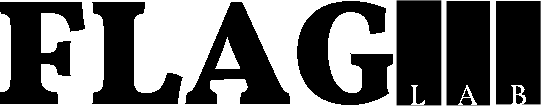
\includegraphics[width=0.6\textwidth]{Flag-logo.png}
                    \end{minipage}%
                    \begin{minipage}{0.55\textwidth}
                        \centering
                        Development of lattice-based abstractions in functional programs\\[1cm]
                        \fontsize{50}{60}
                        \selectfont
                        \textbf{Daniel Barrero${}^1$} \hspace{0.5cm} \textbf{Valérie Gauthier${}^1$} \hspace{0.5cm} \textbf{Nicolás Cardozo${}^1$}\\
                        \fontsize{40}{50}
                        \selectfont
                        ${}^1$Universidad de los Andes\\
                        \texttt{dr.barrero2562@uniandes.edu.co}
                    \end{minipage}%
                    \begin{minipage}{0.25\textwidth}
                    \centering
                        
\includegraphics[width=0.5\textwidth]{logo_uniandes.jpg}
                    \end{minipage}
                    
                };
        \end{tikzpicture}
    \end{center}
    \vspace{2cm}
    \begin{multicols*}{3}
        \fontsize{50}{60}
        \selectfont
        \section{Quantum-safe Cryptography}
        Shor's quantum algorithm, published in 1994, demonstrated that factorization-based cryptography is no longer safe in the face of large-scale quantum computers.
        
        \[
    S_{i,j} =
        \begin{array}{ccccccc}
           \          & \      & |00\rangle & |01\rangle & |10\rangle & |11\rangle & \ \\
           |00\rangle & \vline & 1          & 0          & 0          & 0          & \vline\\
           |01\rangle & \vline & 0          & 1          & 0          & 0          & \vline\\
           |10\rangle & \vline & 0          & 0          & 1          & 0          & \vline\\
           |11\rangle & \vline & 0          & 0          & 0          & e^{i\theta_{k-j}}          & \vline
        \end{array}
\]


    %This begs the question of quantum-safe encryption protocols, for which \emph{the more, the better} rule applies.

    %For instance, the SIDH(KE) protocol was broken in 2022 by an efficient classical algorithm. ----> Have this to mention verbally, as I present the poster.


    % NIST standardization process, and its motivations.



    In 2015, the NSA announced its transition to quantum-resistant algorithms, in recognition of threats such as:

    \begin{enumerate}
        \item Harvesting attacks: store today's keys and cyphertexts to break later.
        \item Forging signatures for old keys.
        \item Implementing new cryptography at scale takes a long time.
    \end{enumerate}

     \vspace{0.2cm}

     
    
\includegraphics[width=0.29\textwidth]{nistComputerSecurity.png}

     Thus began NIST's \emph{PQC standardization} process in 2016, with the following algorithms being winners as of August 2024: \emph{CRYSTALS-kyber, CRYSTALS-dilithium, SPHINCS+ and FALCON.}

 
    \section{Lattice-based cryptography} Of the 4 selected standards, 3 of them rely on Lattice algebra. The reason why this is so practical is that the underlying operations are matrix multiplication and vector addition, unlike the more sophisticated arithmetic of elliptic curve cryptography, for instance. %There is a concern about optimizing the security-level/runtime ratio. \blindtext

    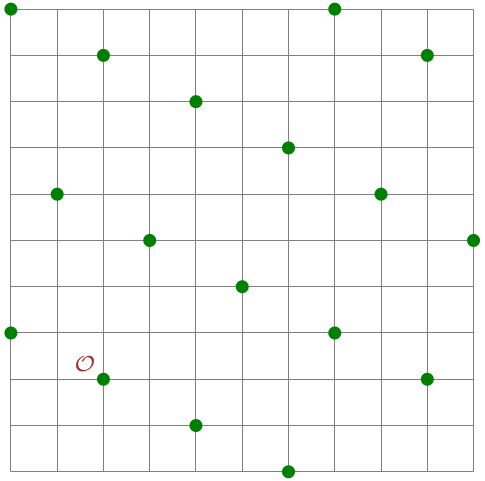
\includegraphics[width=0.20\textwidth]{latticePicture.png}

    Intuitively, a lattice is a periodic grid in space (of arbitrary dimension). More formally, it is the $\mathbb{Z}$-span of a basis for $\mathbb{R}^n$:
    
    \fontsize{45}{45}
    \selectfont
    \[
        L(B) = \{a_1\mathbf{b_1} +...+ a_n\mathbf{b_n} | a_i \in \mathbb{Z}, \mathbf{b_i} \in B\}.
    \]

    \fontsize{50}{60}
    \selectfont

    Computationally hard problems arise when the dimension of the lattice becomes large, the most essential example being the problem of \emph{finding the shortest vector} (SVP, SVP${}_\gamma$). In the related \emph{learning with errors} (LWE) problem, a public key cryptosystem is given by the relation

    \[
        \mathbf{b}^t = \mathbf{s}^t \mathbf{A} + \mathbf{e}^t,
    \]

    where the public key is the random matrix $\mathbf{A}$ and the secret key is the vector $\mathbf{s}$.

    \section{Modern algebra} Advances in mathematics often tend to both simplify and unify seemingly distant theories, as exemplified by the developement of Category Theory since 1945.

    \begin{equation*}
        \begin{tikzcd}
            G \arrow{d}{\nu} \arrow{r}{\alpha} & H \arrow{d}{\mu} \\
            G/G' \arrow{r}{\beta}              & H/H'
        \end{tikzcd}
    \end{equation*}

    \bigskip

    Therefore, with a sufficiently general language, we may attempt to simplify sequences of operations such as those of an encryption scheme. One of such languages is that of operads, whose objects represent \emph{operation composition}.

    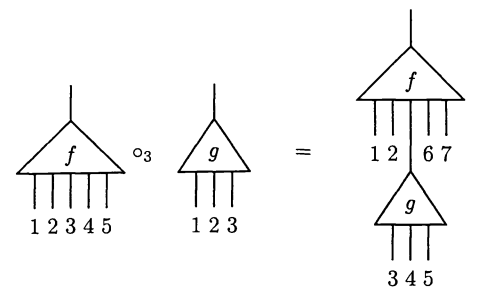
\includegraphics[width=0.29\textwidth]{fig1Intromss02.png}

    Moreover, the fact that standards such as \emph{CRYSTALS-kyber} rely on module theory suggests that applying the aforementioned algebra can yield advantageous simplifications of the current schemes, at least as far as expressing them is concerned.

    % Maybe mention that modern crypto, such as CRYSTALS-Kyber, use module theory? (M_LWE)

    \section{Functional programming} The implementations of the currently selected protocols are written in unsafe languages, such as C and Python. 

    \bigskip
    
    
\includegraphics[width=0.22\textwidth]{haskellLogo.png}

    \bigskip
    
    Meanwhile, functional languages such as Haskell allow programmers to define category-theoretic abstractions in terms of their type system, in a way that is mathematically clear and natural.

    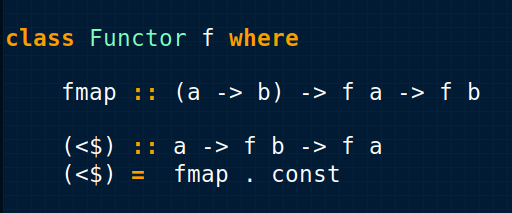
\includegraphics[width=0.29\textwidth]{fctrHskExl.png}

    In this way, we strive to create the language SILVER, %Safely Implemented, Lattice-based Verifiable Encryption Resource.
     which shall have the properties of \textbf{expressibility, safety,} and \textbf{maintainability}. The almost verbatim correspondence between mathematical definitions and type/typeclass declarations in purely functional languages makes this possible (c.f. \emph{Curry-Howard correspondence}), together with the type-check requirement for the execution of a program.

     \begin{minipage}{0.15\textwidth}
         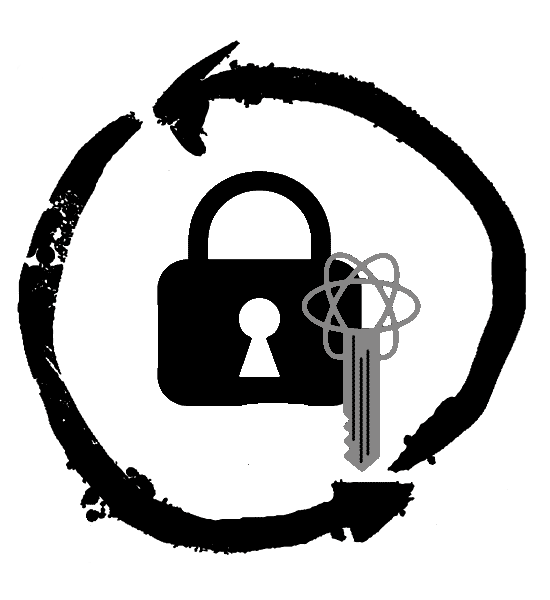
\includegraphics[width=0.5\textwidth]{crypto_0.png}
     \end{minipage}%
     \begin{minipage}{0.15\textwidth}
         
\includegraphics[width=0.5\textwidth]{pil-logo.png}
     \end{minipage}
    
    \end{multicols*}
        
\end{document}